\section{The KAT System Architecture \& Implementation}

\begin{wrapfigure}r{7.6cm}\vspace*{-2em}
  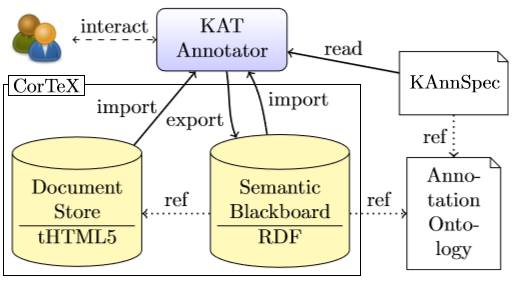
\includegraphics[width=7.6cm]{img/arch}
  \caption{The KAT System Architecture}\label{fig:kat-arch}\vspace*{-1em}
\end{wrapfigure}


As KAT is based on XHTML5, we can employ the XML tool chain and rely on standard libraries for the implementation. In particular, we can use uniform resource identifiers (URI) to identify text fragments and represent annotations in RDF -- subject/predicate/object triples where the components are URI references to web resources. The subjects are usually text fragments, the objects are as well (for relational annotations) or alternatively are concepts from an annotation ontology (for classificational annotations). The predicates are always properties and relations defined in the annotation ontology.

The KAT system itself is realized as a JavaScript library which instruments an XHTML5 document in a browser. To simplify the URI-based referencing of text ranges (node-sets in the HTML document object model) KAT assumes that the document has been word- and sentence-tokenized; the tokens are wrapped in HTML \textsf{span} elements that carry unique \textsf{id} attributes corresponding to the TEI guidelines. The annotation workflow itself is form-based as shown in Figure~\ref{fig:kat-annotate}: the annotator selects a text range, and is then given a modal form to fill classifications and relations as required by the annotation ontology. The annotations are stored as RDF triples in the browser's local storage and can be visualized by special pop-ups and arrows (see Figure~\ref{fig:kat-annotate}).

\begin{figure}[ht]\centering
  %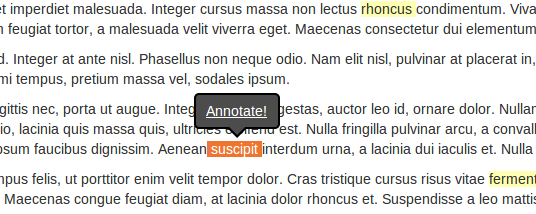
\includegraphics[height=3.2cm]{../papers/PIC/annotate}\quad
  %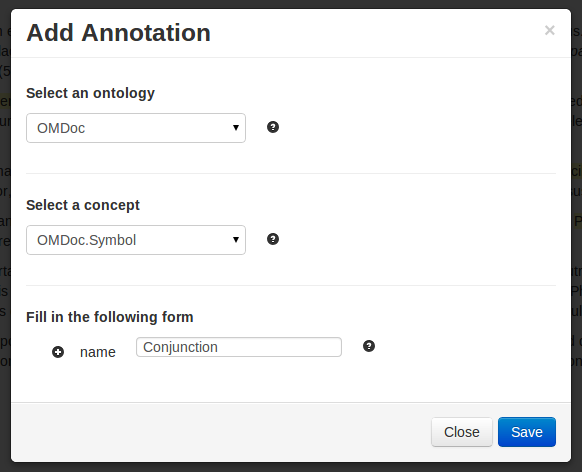
\includegraphics[height=3.1cm]{../papers/PIC/add-symbol}
  \caption{Annotating in KAT: Selection and Form-Filling}\label{fig:kat-annotate}
\end{figure}

KAT is not tied to a particular annotation ontology (or ontology format). At startup, the system is reads a set of \textit{KAT bindings} -- custom XML files that describe the annotation interface, the constraints between the components of an annotation frame, and the RDF to be produced. The frame of OMDoc symbols used in Figure~\ref{fig:kat-annotate}, is given by the fragment of a KAT binding in Listing~\ref{lst:frame}. It specifies
\begin{inparaenum}[\em i\rm)]
\item the fields of the annotation form, their values and validation constraints,
\item their display, and
\item the RDF subgraph for the frame via a templating mechanism.
\end{inparaenum}
Note that this frame classifies the annotated word as an OMDoc symbol (via the \lstinline [basicstyle=\sf\normalsize]|rdf:type| predicate) and relates it to its name via the \lstinline[basicstyle=\sf\normalsize]|o:symbolname| relation from the OMDoc ontology.

\begin{lstlisting}[language=XML,label=lst:frame,
caption=A KAT Frame Specification for OMDoc Symbols]
<frame name="Symbol">
    <help>An OpenMath/OMDoc Symbol</help>
    <fields>
        <field name="name" type="text">
            <help>The name of the symbol defines it in a theory</help>
            <value>Name</value>
            <default>Symbol</default>
            <validation>[A-Z][a-z]*</validation>
        </field>
    </fields>
    <display> ... </display>
    <rdf:RDF xmlns:rdf="http://www.w3.org/1999/02/22-rdf-syntax-ns#">
        <rdf:Description xmlns:o="http://omdoc.org/ontology#">
            <rdf:type rdf:resource="http://omdoc.org/ontology#Symbol"/>
            <o:symbolname>{name}</o:symbolname>
        </rdf:Description>
    </rdf:RDF>
</frame>
\end{lstlisting} \ednote{Update and redo KAnnSpecs}

Even though KAT can work as a standalone library that can be added to any STEM document in HTML5, it is best used as a component of a corpus management system, such as the {Cor\TeX} system~\cite{CorTeX:on} developed by the second author. In this situation the annotator requests an annotation task from {Cor\TeX}, which serves the TEI-tokenized document with KAT and a set of bindings for the intended annotation ontologies. When the annotation is complete, the generated RDF is exported to the semantic blackboard -- an RDF triple store maintained by {Cor\TeX}. When combined with {Cor\TeX}, KAT can be used by multiple annotators; and can be used to review existing annotations, by importing them from the triple store.  KAT also has experimental support for inter-annotator agreement reviews via a side-by-side view of the various annotations.

\ednote{UI Implementaton}
